\documentclass{article}
\usepackage[linesnumbered,ruled,vlined]{algorithm2e}
\usepackage{pgfplots}
\usepackage{amsmath}
\pgfplotsset{compat=1.18}

\begin{document}
\section{What is a Neural Network?}

A neural network is a computational model inspired by the structure of the human brain, designed to recognize patterns and make predictions by learning from data. It consists of layers of interconnected nodes (neurons) that transform input data through weighted connections and activation functions to produce outputs. For this neural network, rather than having the weights randomly assigned and the ANN gradually changing them itself, I have input multiple weights as to play around adn understand what chanign each weight does and why some are better and some are worse.

\section{Weights Explanation}
The parameters in this ANN are input size, hidden size, eta, output size, and iterations. The input size and the output size are set as each piece of data in the iris set has four components meaning four inputs and there are only three types of iris each data point can be meaning there can only be three outputs. 
\subsection{Hidden size} 
Hidden size determines how many neurons are in the hidden layer and they mark how much complexity the network can take in. For example in this ANN I tried using 2 and that was insufficient for geting good results while using 20 caused overfitting. I found 6 to be a good amount of hidden layers.
\subsection{ETA} 
Eta represents the learning rate and controls how big each weight adjustment is during the training. I settled on 0.04 for the eta as it was precise when the amount of iterations was sufficient. 0.01 for the eta resulted in poor percentages well under 50 percent while using an eta like 5.00 resulted in high learning speed but massive differences between each iteration with lots of inconcistencies and not a gradual display of the learning. 
\subsection{Iterations} 
The number of iterations determines how many times the network processes the training data allowing it to gradually define weights and improve accuracy. In this ANN I created a loop that uses iterations as little as 10 and as much as 10,000. 10 iterations was insufficent and lead to poor accuracy while 10,000 did the same. The best amount of iterations for this model came from the the middle values which resulted in high accuracy while avoiding overfitting.
\subsection{What is Overfitting?}
Overfitting occurs when a neural network learns the training data too well, capturing not only the underlying patterns but also the random noise and outliers. This makes the model perform exceptionally on the training set but poorly on new, unseen data because it fails to generalize beyond what it has memorized. Overfitting typically happens when the model is too complex relative to the amount of data available, such as having too many layers or neurons. For example in this ANN, I found that overfitting occured when there were too many hidden layers or too many iterations. This resulted in the accuracy coming back at over 100 percent meaning that the network was not generalizing beyond what it has memorized and given new data points would perform extremely poorly.


\begin{algorithm}[H]
\caption{Training Multiple ANN Models with Different Iterations}
\KwData{Training data $X_{train}$, training labels $y_{train}$}
\KwIn{$input\_size = 4$, $hidden\_size = 6$, $output\_size = 3$, $learning\ rate\ \eta = 0.04$}
\KwOut{Trained artificial neural networks for each iteration count}

Define list of iteration counts: $N \leftarrow [10, 100, 500, 1000, 1500, 2500, 5000, 10000]$\;
\ForEach{$n_i$ in $N$}{
    Initialize ANN model with parameters $(input\_size, hidden\_size, output\_size, \eta, n_i)$\;
    Train the model using $ANN.fit(X_{train}, y_{train})$\;
    Print ``done'' to indicate training completion\;
}
\end{algorithm}
This algorithm is the for loop I created to run the model with multiple iterations to test what would be around the best for getting a high accuracy.

\begin{algorithm}[H]
\SetAlgoLined
\caption{Training the Neural Network via Backpropagation}
\KwIn{Input data $X$, true labels $y$, learning rate $\eta$, number of iterations $n_{\text{iter}}$}
\KwOut{Updated weights $W_1, W_2$ and biases $b_1, b_2$}

\For{$i \leftarrow 1$ \KwTo $n_{\text{iter}}$}{
    \tcc{Forward pass}
    $h_{\text{in}} \leftarrow X \cdot W_1 + b_1$ \\
    $h_{\text{out}} \leftarrow \sigma(h_{\text{in}})$ \\
    $f_{\text{in}} \leftarrow h_{\text{out}} \cdot W_2 + b_2$ \\
    $f_{\text{out}} \leftarrow \sigma(f_{\text{in}})$ \\

    \tcc{Compute error}
    $\text{error} \leftarrow y - f_{\text{out}}$ \\

    \tcc{Backward pass}
    $\delta_f \leftarrow \text{error} \times \sigma'(f_{\text{out}})$ \\
    $\text{error}_h \leftarrow \delta_f \cdot W_2^T$ \\
    $\delta_h \leftarrow \text{error}_h \times \sigma'(h_{\text{out}})$ \\

    \tcc{Update weights and biases}
    $W_2 \leftarrow W_2 + h_{\text{out}}^T \cdot \delta_f \times \eta$ \\
    $b_2 \leftarrow b_2 + \sum(\delta_f) \times \eta$ \\
    $W_1 \leftarrow W_1 + X^T \cdot \delta_h \times \eta$ \\
    $b_1 \leftarrow b_1 + \sum(\delta_h) \times \eta$ \\
}

\end{algorithm}
This algorithm basically takes the parameters and weights and completes backpropogation then updating the weights and biases

\begin{algorithm}[H]
\SetAlgoLined
\caption{Predict Function for Neural Network}
\label{algo:predict}
\KwIn{Input data $X$, trained weights $W_1, W_2$, and biases $b_1, b_2$}
\KwOut{Predicted class labels}

\tcc{Forward pass through the network}
$h_{\text{in}} \leftarrow X \cdot W_1 + b_1$ \\
$h_{\text{out}} \leftarrow \sigma(h_{\text{in}})$ \\
$f_{\text{in}} \leftarrow h_{\text{out}} \cdot W_2 + b_2$ \\
$f_{\text{out}} \leftarrow \sigma(f_{\text{in}})$ \\

\tcc{Determine predicted classes}
$\text{predictions} \leftarrow \arg\max(f_{\text{out}}, \text{axis}=1)$ \\

\Return $\text{predictions}$

\end{algorithm}

This algorithm (algorithm \ref{alg:predict}) takes the input feature matrix, trained weight matrices, trained bias vectors, sigmoid activation function, and then selects the index of the neuron with the highest activation for each. Then predicting the result.


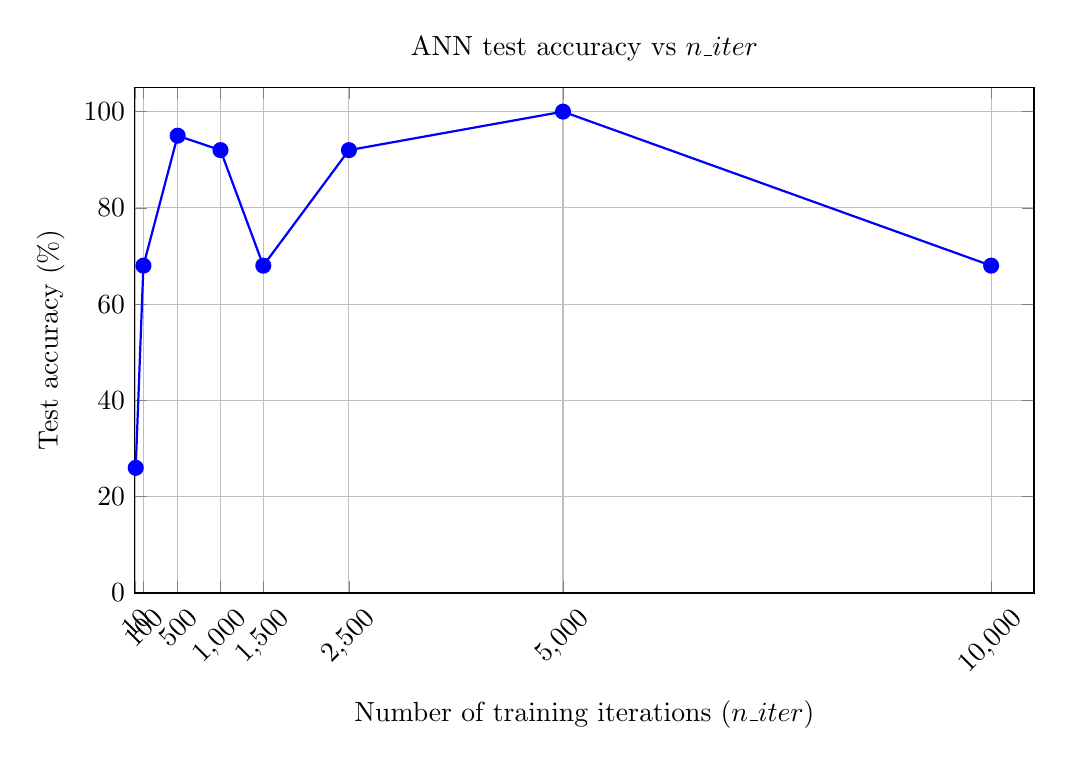
\begin{tikzpicture}
\begin{axis}[
    width=13cm,
    height=8cm,
    xlabel={Number of training iterations ($n\_iter$)},
    ylabel={Test accuracy (\%)},
    title={ANN test accuracy vs $n\_iter$},
    grid=major,
    ymin=0, ymax=105,
    xmin=0, xmax=10500,
    xtick={10,100,500,1000,1500,2500,5000,10000},
    xticklabel style={rotate=45},
    scaled x ticks=false,
    ytick={0,20,40,60,80,100},
    mark size=2.5pt 
]

\addplot[
    color=blue,
    mark=*,
    thick
] coordinates {
    (10,26)
    (100,68)
    (500,95)
    (1000,92)
    (1500,68)
    (2500,92)
    (5000,100)
    (10000,68)
};

\end{axis}
\end{tikzpicture}
This plot displays how the accuracy ended up with each value of iterations in the for loop. 

\section{Final Thoughts}
Over the course of the last week I adapted and ran this code over 100 times and was unable to find complete consistency. Regardless of how I changed the weights, sometimes iterations would perform incredibly poorly and leave random spikes where I do not think they should have. There was consistency with the 10, 100, and 500 iteration amounts all being poor but with the greater iterations it seemed to not have a consistent pattern and it was difficult to find what the correct amount of iterations would be. I would guess it to be somewhere between 1000 and 2500 but sometimes that middleground would perform poorly. After running the same could upwards up 10 times as well things would begin to plateau and then suddenly change completely with no change done to the source code. At this point, these are where my questions lie and I am eager to learn more and figure out why that may be since I think I have a decent understadnign of how the weights and overfitting works.
\end{document}


